\documentclass[11pt]{article}

\usepackage[margin=1in]{geometry}
\usepackage{amsmath, amssymb, amsthm}
\usepackage{mathtools}
\usepackage{bm}
\usepackage{graphicx}
\usepackage{tikz}
\usetikzlibrary{positioning, arrows.meta, fit, calc, backgrounds, shapes.geometric}
\usepackage{booktabs}
% --- minimal home-grown algorithm pseudocode (no algorithm package available) ---
\usepackage{verbatim}
\newcounter{algocounter}
\newenvironment{algorithm}[1][h]{\par\refstepcounter{algocounter}%
  \begin{quote}\small\noindent\textbf{Algorithm \thealgocounter:}\quad\ignorespaces}
  {\end{quote}\par}
\newcommand{\Require}{\par\noindent\textbf{Input:}\ \ignorespaces}
\newcommand{\Comment}[1]{\quad\(\triangleright\) \textit{#1}}
\newcommand{\Return}{\par\noindent\textbf{Return:}\ \ignorespaces}
\newcommand{\State}{\par\noindent\hspace*{1em}}
\usepackage{hyperref}
\usepackage{xcolor}
\usepackage[numbers, square]{natbib}

\newcommand{\xE}{\vec{x}_E}
\newcommand{\xP}{\vec{x}_P}
\newcommand{\vE}{\vec{v}_E}
\newcommand{\vP}{\vec{v}_P}
\newcommand{\uE}{\hat{u}_E}
\newcommand{\uP}{\hat{u}_P}
\newcommand{\TT}{\mathbb{T}^{2}}
\newcommand{\RR}{\mathbb{R}}
\newcommand{\NN}{\mathbb{N}}
\newcommand{\E}{\mathbb{E}}

\title{\bf Learning Embeddings of Pursuit--Evasion Strategies on the
            Torus via Adversarial Multi-Head Networks}
\author{}
\date{May 2026}

\begin{document}
\maketitle

\begin{abstract}
We adapt the multi-head Physics-Informed Neural Network framework of
Jimenez et al.\ for learning low-dimensional embeddings of PDE solution
families to a class of \emph{differential games}: a two-player
pursuit--evasion game on the periodic flat torus $\TT=[0,L)^2$.
Two networks, one per player, share a body MLP that maps time
$t\in[0,t_{\max}]$ to a latent representation $H_\alpha(t)\in\RR^{n_b}$,
while $N_h$ linear heads --- one per initial position of the evader ---
linearly combine the latent components and project onto the unit circle
$\mathbb{S}^1$ to produce the player's instantaneous direction of motion.
We derive the underlying Hamilton--Jacobi--Isaacs (HJI) equation, recast
the resulting min--max problem as an adversarial training objective with
a differentiable expected first-capture time built from a smooth survival
function, and integrate trajectories on the torus with explicit
periodicity.  The two networks are trained adversarially via alternating
gradient steps with a pursuer-favoured step ratio $k_P\!:\!k_E\!=\!2\!:\!1$
and a short single-player pre-training warm-up for the pursuer.
A reference PyTorch implementation and a self-contained NumPy
implementation with hand-coded forward and backward passes
(validated against finite differences to $\sim 10^{-8}$ relative error)
are provided.  Numerical experiments on a $12$-initial-condition setup
demonstrate that the learned strategies recover the qualitative
behaviour expected from the geometry of the homicidal-chauffeur game on
a periodic domain.  The embedding lens carried over from PDE solution
manifolds suggests a natural notion of an
``optimal-strategy manifold'' for differential games.
\end{abstract}

\tableofcontents

%=============================================================================
\section{Introduction}
%=============================================================================
Differential games \citep{Isaacs1965} provide the natural language for
multi-agent decision problems whose state and controls evolve in continuous
time.  The canonical example is the pursuit--evasion game: a faster
\emph{pursuer} tries to minimise the time at which its position
coincides (up to a capture radius) with that of the \emph{evader}, who
in turn tries to maximise this time.  Closed-form solutions are known
only for special geometries
\citep{Isaacs1965, basar1999dynamic, lewin2012differential};
in general one must solve the Hamilton--Jacobi--Isaacs (HJI) PDE for
the upper- and lower-value functions of the game, a problem that is
notoriously affected by the curse of dimensionality.

A recent line of work has applied physics-informed and operator-learning
neural networks to such variational problems
(see Section~\ref{sec:lit} for a survey).  In parallel, Jimenez et al.\
\citep{JimenezEmbeddings2026} have shown that, for nonlinear PDEs such
as the Burgers, heat and wave equations, a \emph{multi-head}
physics-informed architecture --- a shared body MLP and a bank of
linear, orthogonality-penalised heads, one per initial condition ---
learns a finite-dimensional embedding of the solution manifold whose
principal components are stable across training realisations.
This paper adapts that construction to differential games on a periodic
domain.

The choice of the torus $\TT$ is deliberate: it removes confounding
boundary effects, makes the system translation-equivariant under the
diagonal action of $\TT$, and matches the setting of many turbulent or
cosmological reductions in which the embeddings framework has been
analysed.  All vector identities used below admit unambiguous
torus interpretations as long as quantities are written in terms of
minimum-image displacements.

%-----------------------------------------------------------------------------
\paragraph{Contributions.}
\begin{enumerate}
\item A self-contained derivation of the HJI equation for the
      pursuit--evasion game on $\TT$, including saddle-point feedback
      controls (Section~\ref{sec:hji}).
\item A multi-head, time-parametrised adversarial architecture that
      mirrors the embeddings construction of~\citep{JimenezEmbeddings2026}
      and produces unit-direction outputs in $\mathbb{S}^1$
      (Section~\ref{sec:arch}).
\item A differentiable expected first-capture-time loss built from a
      smooth survival function, combined with a zero-sum distance
      shaping term that prevents gradient vanishing in the no-capture
      regime (Section~\ref{sec:loss}).
\item A reference PyTorch implementation and a NumPy implementation with
      hand-coded forward/backward passes (Section~\ref{sec:impl},
      Appendix~\ref{app:gradcheck}).
\item Numerical experiments illustrating the learned trajectories,
      heading-angle profiles, and the PCA spectrum of the latent
      embeddings $H_\alpha(t)$ (Section~\ref{sec:experiments}).
\end{enumerate}

%=============================================================================
\section{Game setup}
\label{sec:setup}
%=============================================================================
Let $L>0$ and set the domain to the flat torus
$\TT \coloneqq (\RR/L\RR)^2$ with the canonical projection
$\pi:\RR^2\to\TT$.  Distances on $\TT$ are minimum-image distances:
\begin{equation}
\|\vec{a} - \vec{b}\|_\TT
  \;\coloneqq\;
  \big\| \big((\vec{a}-\vec{b}) + L/2\big) \bmod L \;-\; L/2 \big\|_{\RR^2}.
\end{equation}
We use the symbol $\Delta_\TT(\vec{a},\vec{b})$ for the signed
minimum-image displacement,
$\Delta_\TT(\vec{a},\vec{b}) \in [-L/2,L/2)^2$, so that
$\|\vec{a}-\vec{b}\|_\TT = \|\Delta_\TT(\vec{a},\vec{b})\|$.

\smallskip

The state of the game at time $t\in[0,t_{\max}]$ is the pair
$\big(\xE(t),\xP(t)\big)\in\TT\times\TT$.  The dynamics are
\begin{equation}
\label{eq:dyn}
\dot{\xE}(t) \;=\; v_E\,\uE(t), \qquad
\dot{\xP}(t) \;=\; v_P\,\uP(t),
\qquad \uE,\uP\in\mathbb{S}^{1},
\end{equation}
with fixed speeds
\begin{equation}
v_E \;=\; 1, \qquad v_P \;=\; a > 1.
\end{equation}
We adopt $a=1.2$ throughout.  Without loss of generality (by torus
translation invariance) the pursuer is initialised at the origin,
$\xP(0)=(0,0)$, and the evader's initial position $\xE(0)$ is treated
as a parameter of the game.  Capture is declared at the first time
\begin{equation}
T_c \;\coloneqq\; \inf\big\{\, t\ge 0 \,:\,
                  \|\xE(t)-\xP(t)\|_\TT \le \varepsilon \,\big\},
\end{equation}
where $\varepsilon>0$ is a (small) capture radius.  If the infimum is
empty in $[0,t_{\max}]$, we set $T_c = t_{\max}$ by convention.

%=============================================================================
\section{Hamilton--Jacobi--Isaacs derivation}
\label{sec:hji}
%=============================================================================
We derive the Bellman--Isaacs equation for the (upper) value
function of the game, following the standard treatment for two-player
zero-sum differential games \citep{Isaacs1965, basar1999dynamic,
elliotkalton1972}.

\subsection{Value function}
Define the value of the game starting from a state
$\vec{x} = (\xE,\xP)\in\TT\times\TT$ outside the capture set
$\mathcal{C}_\varepsilon\coloneqq \{(\xE,\xP):\|\xE-\xP\|_\TT\le\varepsilon\}$
as the time to capture under optimal play of both sides:
\begin{equation}
V(\vec{x})
\;\coloneqq\;
\inf_{\uP(\cdot)} \sup_{\uE(\cdot)}
T_c(\vec{x};\uP(\cdot),\uE(\cdot)).
\end{equation}
On the boundary of the capture set, $V \equiv 0$.

\subsection{Bellman--Isaacs principle}
Standard dynamic-programming arguments \citep{evans1984differential,
basar1999dynamic} yield, for any $\delta t>0$ such that the trajectories
remain outside $\mathcal{C}_\varepsilon$,
\begin{equation}
V(\vec{x})
\;=\;
\inf_{\uP}\sup_{\uE}
\;
\big[\delta t \;+\; V(\vec{x}+\delta t\,f(\vec{x};\uE,\uP))\big]
\;+\; o(\delta t),
\end{equation}
where $f(\vec{x};\uE,\uP) = (v_E \uE,\,v_P \uP)$.  Taylor-expanding and
dividing by $\delta t$,
\begin{equation}
\label{eq:HJI-pre}
\inf_{\uP\in\mathbb{S}^1}\sup_{\uE\in\mathbb{S}^1}
\bigl\{
v_E\,\nabla_{\xE}V\cdot\uE
\;+\;
v_P\,\nabla_{\xP}V\cdot\uP
\bigr\}
\;+\; 1
\;=\; 0.
\end{equation}
Because $V$ is intrinsically a function on $\TT\times\TT$, the gradients
$\nabla_{\xE},\nabla_{\xP}$ are computed on the torus (they are the
ordinary partial derivatives evaluated on the periodic lift).
The Isaacs minimax condition holds because the Hamiltonian is separable
in $\uE$ and $\uP$, so $\inf_{\uP}\sup_{\uE} = \sup_{\uE}\inf_{\uP}$.

\subsection{Saddle-point controls}
Eq.~\eqref{eq:HJI-pre} is solved analytically in $\uE,\uP$ because each
term is linear in the control.  For the supremum over $\uE\in\mathbb{S}^1$,
\begin{equation}
\sup_{\uE\in\mathbb{S}^1} v_E\,\nabla_{\xE}V\cdot\uE
\;=\;
v_E\,\|\nabla_{\xE}V\|,
\qquad
\uE^\star \;=\; \frac{\nabla_{\xE}V}{\|\nabla_{\xE}V\|}.
\end{equation}
For the infimum over $\uP\in\mathbb{S}^1$,
\begin{equation}
\inf_{\uP\in\mathbb{S}^1} v_P\,\nabla_{\xP}V\cdot\uP
\;=\;
-v_P\,\|\nabla_{\xP}V\|,
\qquad
\uP^\star \;=\; -\frac{\nabla_{\xP}V}{\|\nabla_{\xP}V\|}.
\end{equation}
Substituting back into~\eqref{eq:HJI-pre} gives the
\emph{Hamilton--Jacobi--Isaacs equation} for the pursuit--evasion game
on $\TT$:
\begin{equation}
\label{eq:HJI}
\boxed{\;
v_E\,\|\nabla_{\xE}V\| \;-\; v_P\,\|\nabla_{\xP}V\| \;+\; 1 \;=\; 0
\;}
\qquad \text{on } (\TT\times\TT)\setminus\mathcal{C}_\varepsilon,
\end{equation}
with boundary condition $V = 0$ on $\partial\mathcal{C}_\varepsilon$.

\noindent
Equivalently, in the residual form used in the board-derivation of the
project brief,
\begin{equation}
\mathcal{R}(V) \;\coloneqq\;
- v_P\,\|\nabla_{\xP}V\| \;+\; v_E\,\|\nabla_{\xE}V\| \;-\; 1 \;=\; 0.
\end{equation}

\subsection{Open-loop reformulation}
The HJI~\eqref{eq:HJI} is the standard \emph{feedback} (closed-loop)
formulation: the optimal control of each player at the present time
depends on the present state via the gradients of $V$.  In this work we
follow the project specification and instead train networks that
produce \emph{open-loop} controls
$\uE(t),\uP(t)$ as functions of time alone, parametrised by the initial
condition of the evader through the choice of head.  Because the system
is fully deterministic and the open-loop Nash equilibrium of a
zero-sum game with continuous compact-valued controls coincides with
the closed-loop one whenever Isaacs' condition holds
\citep{basar1999dynamic, elliotkalton1972}, the open-loop networks are
in principle expressive enough to recover the HJI saddle point.  The
practical price is that learning is sensitive to the initial condition,
which motivates the multi-head architecture below.

%=============================================================================
\section{Multi-head adversarial architecture}
\label{sec:arch}
%=============================================================================
For each player $\alpha\in\{E,P\}$ we construct a neural network
\begin{equation}
\mathcal{N}_\alpha:
\quad
t\in[0,t_{\max}]
\;\longmapsto\;
\bigl(\hat{u}_\alpha^{1}(t),\dots,\hat{u}_\alpha^{N_h}(t)\bigr)
\in (\mathbb{S}^1)^{N_h}.
\end{equation}
The architecture mirrors the multi-head design
of~\citep{JimenezEmbeddings2026}: a \emph{shared body} produces a latent
embedding $H_\alpha(t)\in\RR^{n_b}$ common to all initial conditions of
the evader, and $N_h$ \emph{linear heads} specialise this embedding to
the $j$-th initial condition.  Concretely,
\begin{align}
\phi(t)
&\;\coloneqq\;
\big[\sin(\omega_k t),\,\cos(\omega_k t),\,t/t_{\max}\big]_{k=1}^{K},
\quad \omega_k = \frac{2\pi k}{t_{\max}},
\label{eq:phi}\\[2pt]
H_\alpha(t)
&\;=\;
\mathrm{MLP}_\alpha(\phi(t);\,\theta_\alpha^{\rm body}),
\qquad H_\alpha(t)\in\RR^{n_b},
\label{eq:body}\\[2pt]
z_\alpha^{j}(t)
&\;=\;
W_\alpha^{j} \, H_\alpha(t),
\qquad W_\alpha^{j}\in\RR^{2\times n_b},
\label{eq:head}\\[2pt]
\hat{u}_\alpha^{j}(t)
&\;=\;
\frac{z_\alpha^{j}(t)}{\|z_\alpha^{j}(t)\|},
\qquad
\vec{v}_\alpha^{j}(t)
\;=\;
v_\alpha\,\hat{u}_\alpha^{j}(t).
\label{eq:unit}
\end{align}
Eq.~\eqref{eq:phi} is the time-encoding analogue of the spatial Fourier
features used in the PDE embeddings paper.  Eq.~\eqref{eq:head} is the
linear head whose weights identify the initial condition.
Eq.~\eqref{eq:unit} projects onto $\mathbb{S}^1$ so that the velocity
norm is exactly the fixed speed of each player.
The reference PyTorch implementation uses a four-layer Tanh MLP body of
width $128$ for~\eqref{eq:body}; the NumPy reference implementation
uses a one-layer Tanh body (linear $\to$ tanh), which is sufficient for
the experiments below and admits closed-form gradients.

\medskip

\paragraph{Head orthogonalisation.}  Following
\citep{JimenezEmbeddings2026}, we add a penalty
\begin{equation}
\label{eq:head-orth}
L_\alpha^{\rm orth}
\;=\;
\big\| W_\alpha W_\alpha^\top - I\big\|_F^2
+\big\| W_\alpha^\top W_\alpha - I\big\|_F^2,
\end{equation}
where $W_\alpha\in\RR^{(2N_h)\times n_b}$ is the flattened head matrix.
This penalty discourages collapse of the latent space onto a
lower-rank subspace and stabilises the principal-component spectrum of
$H_\alpha$ across training seeds; it is a direct adaptation of the
PCA-stability device in the PDE embeddings paper.  We set the
coefficient $\lambda_{\rm orth} = 10^{-4}$ in our experiments; it is
small enough that the residual game loss dominates.

\medskip

\begin{figure}[h]
\centering
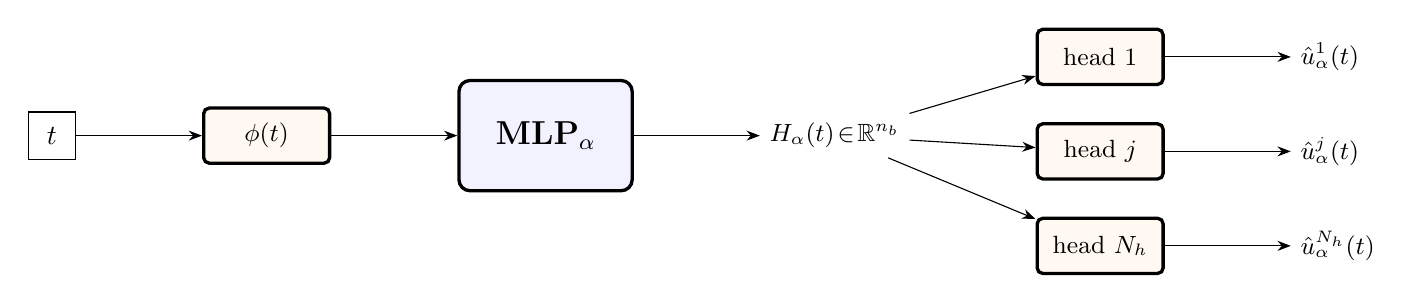
\begin{tikzpicture}[
    >=Stealth,
    node distance=1.0cm and 1.6cm,
    nn/.style={draw, very thick, rounded corners=4pt,
               minimum width=2.2cm, minimum height=1.4cm,
               font=\large\bfseries, fill=blue!5},
    box/.style={draw, very thick, rounded corners=2pt,
                minimum width=1.6cm, minimum height=0.7cm,
                font=\small, fill=orange!5},
    inp/.style={draw, minimum width=0.6cm, minimum height=0.6cm,
                fill=white},
]
\node[inp] (t) at (0,0) {$t$};
\node[box, right=of t] (phi) {$\phi(t)$};
\node[nn, right=of phi] (body) {MLP$_\alpha$};
\node[right=of body, font=\small] (Halpha) {$H_\alpha(t)\!\in\!\RR^{n_b}$};
\node[box, right=of Halpha, yshift=10mm] (h1) {head $1$};
\node[box, right=of Halpha, yshift=-2mm] (h2) {head $j$};
\node[box, right=of Halpha, yshift=-14mm] (h3) {head $N_h$};
\node[right=of h1, font=\small] (u1) {$\hat u_\alpha^{1}(t)$};
\node[right=of h2, font=\small] (u2) {$\hat u_\alpha^{j}(t)$};
\node[right=of h3, font=\small] (u3) {$\hat u_\alpha^{N_h}(t)$};
\draw[->] (t) -- (phi);
\draw[->] (phi) -- (body);
\draw[->] (body) -- (Halpha);
\foreach \hh/\out in {h1/u1, h2/u2, h3/u3} {
    \draw[->] (Halpha) -- (\hh);
    \draw[->] (\hh) -- (\out);
}
\end{tikzpicture}
\caption{Multi-head time-dependent velocity network for one player
$\alpha\in\{E,P\}$.  A single MLP body produces the latent embedding
$H_\alpha(t)$.  Each of the $N_h$ linear heads is associated with one
initial condition of the evader and outputs the player's
instantaneous unit direction after projection on $\mathbb{S}^1$.
A symmetric network is trained for the opposite player.}
\label{fig:arch}
\end{figure}

%=============================================================================
\section{Trajectory rollout and loss}
\label{sec:loss}
%=============================================================================
\subsection{Rollout on the torus}
We discretise time uniformly,
$t_k = k\,\Delta t$, $k=0,\dots,N_t$, with $\Delta t = t_{\max}/N_t$,
and integrate~\eqref{eq:dyn} with an explicit trapezoidal step composed
with the canonical projection $\pi:\RR^2\to\TT$:
\begin{equation}
\label{eq:rollout}
\begin{aligned}
\xi^j_{E,k+1}
&\;=\;
\pi\!\left(\xi^j_{E,k} + \Delta t\, v_E\,
\tfrac{1}{2}\!\big(\hat u^{j}_{E}(t_k)+\hat u^{j}_{E}(t_{k+1})\big)\right), \\
\xi^j_{P,k+1}
&\;=\;
\pi\!\left(\xi^j_{P,k} + \Delta t\, v_P\,
\tfrac{1}{2}\!\big(\hat u^{j}_{P}(t_k)+\hat u^{j}_{P}(t_{k+1})\big)\right),
\end{aligned}
\end{equation}
with $\xi^j_{P,0} = 0$ and $\xi^j_{E,0} = \xE^{(j)}(0)$, $j=1,\dots,N_h$.
The midpoint average makes the step second-order accurate in $\Delta t$
even though the velocities are evaluated at the endpoints.  The
projection $\pi$ is implemented as the componentwise residue modulo
$L$ and has gradient equal to the identity in the interior, which is
the case we encounter except on a set of Lebesgue measure zero.

\subsection{Smooth survival function and expected first-capture time}
Define the per-step squared minimum-image distance
$d^{j}_{k}\,^2 \coloneqq \|\Delta_\TT(\xi^j_{E,k},\xi^j_{P,k})\|^2$,
and the per-step soft capture probability
\begin{equation}
p^j_k \;=\; \sigma\!\left(\frac{\varepsilon^2 - d^j_k\,^2}{\tau}\right),
\qquad \sigma(x) = (1+e^{-x})^{-1}.
\end{equation}
The cumulative \emph{survival} probability is
\begin{equation}
S^j_k \;=\; \prod_{l=0}^{k} (1 - p^j_l)
       \;=\; \exp\Big(\sum_{l=0}^{k} \log(1-p^j_l)\Big),
\end{equation}
implemented via $\log(1-\sigma(x)) = -\mathrm{softplus}(x)$ for numerical
stability.  For a non-negative random variable $T_c$,
$\E[T_c]=\int_0^\infty \Pr(T_c>t)\,dt$, which we approximate by the
trapezoidal rule on the time grid:
\begin{equation}
\E[T_c]^{j}_{\rm soft}
\;\approx\;
\Delta t\!\left(
\tfrac{1}{2}S^j_0 + \sum_{k=1}^{N_t-1} S^j_k + \tfrac{1}{2} S^j_{N_t}
\right).
\end{equation}
This quantity is differentiable in all positions $\xi^j_{\alpha,k}$ and
hence in all network weights through~\eqref{eq:rollout}.

\subsection{Adversarial losses}
The pursuer minimises and the evader maximises the expected
first-capture time.  Two practical considerations force us to augment
this objective.  First, when the trajectories are far from the capture
set, $p^j_k\to 0$ and the gradient of $\E[T_c]_{\rm soft}$ through the
$\sigma$ saturates: an open-loop network initialised at random has no
gradient signal to know in which direction to head.  Second, we want
to penalise the pursuer explicitly when capture fails altogether
$(S^j_{N_t}\!>\!0)$.

We therefore use a composite loss
\begin{align}
\label{eq:LP}
\mathcal{L}_P &\;=\; \overline{\E[T_c]}_{\rm soft}
 \;+\; \lambda_{\rm nc}\,\overline{S^j_{N_t}}\,t_{\max}
 \;+\; \lambda_d\,\overline{\langle d \rangle}, \\
\label{eq:LE}
\mathcal{L}_E &\;=\;
 -\,\overline{\E[T_c]}_{\rm soft}
 \;-\; \lambda_d\,\overline{\langle d \rangle},
\end{align}
where overlines denote the empirical mean over the $N_h$ heads and
$\langle d \rangle^j = \tfrac{1}{N_t+1}\sum_k \|\Delta_\TT(\xi^j_E,\xi^j_P)_k\|$.
The third term $\lambda_d\langle d\rangle$ is a \emph{zero-sum} distance
shaping that always provides a non-vanishing gradient (since
$\|\partial \|\Delta\|/\partial \Delta\| = 1$ outside the origin) and is
applied with opposite signs to the two players.  Setting
$\lambda_d=0$ recovers the pure first-capture-time game; we take
$\lambda_d=5$ and $\lambda_{\rm nc}=2$ in the experiments below.

\subsection{Algorithm}
Algorithm~\ref{alg:pursuit} summarises the training loop.  A short
single-player pursuer warm-up
($\sim 800$ steps against the randomly initialised evader) makes the
subsequent adversarial phase substantially more stable; without it
adversarial dynamics frequently collapse to the no-capture corner.

\begin{algorithm}[h]
\textbf{Adversarial training of the multi-head pursuit--evasion networks
on $\TT$.}\par\smallskip
\Require initial-condition set $\{\xE^{(j)}(0)\}_{j=1}^{N_h}$;
hyperparameters $v_E,v_P,L,\varepsilon,\tau,t_{\max},N_t,
\lambda_d,\lambda_{\rm nc},\lambda_{\rm orth},$
learning rates $\eta_E,\eta_P$, step ratio $k_P\!:\!k_E$.
\begin{enumerate}\setlength{\itemsep}{0pt}
  \item Initialise $\theta_E,\theta_P$, Adam optimisers
        $\mathcal{A}_E,\mathcal{A}_P$.
  \item \textbf{Pursuer warm-up.}  For $i = 1,\dots,i_{\rm warm}$:
        $\theta_P\!\leftarrow\!\theta_P-\eta_P\,\mathcal{A}_P\!
        \big(\nabla_{\theta_P}(\mathcal{L}_P+\lambda_{\rm orth}L^{\rm orth}_P)\big).$
  \item \textbf{Adversarial phase.} For $i = 1,\dots,i_{\max}$:
        \begin{enumerate}
          \item Repeat $k_P$ times: forward roll
            $\xi^j_E,\xi^j_P$ via~\eqref{eq:rollout}; compute
            $\mathcal{L}_P$;
            $\theta_P\!\leftarrow\!\theta_P-\eta_P\,\mathcal{A}_P\!
            \big(\nabla_{\theta_P}(\mathcal{L}_P+\lambda_{\rm orth}L^{\rm orth}_P)\big).$
          \item Repeat $k_E$ times: forward roll; compute $\mathcal{L}_E$;
            $\theta_E\!\leftarrow\!\theta_E-\eta_E\,\mathcal{A}_E\!
            \big(\nabla_{\theta_E}(\mathcal{L}_E+\lambda_{\rm orth}L^{\rm orth}_E)\big).$
        \end{enumerate}
  \item \Return $(\theta_E,\theta_P)$.
\end{enumerate}
\label{alg:pursuit}
\end{algorithm}

%=============================================================================
\section{Implementation}
\label{sec:impl}
%=============================================================================
We provide two reference implementations.

\paragraph{PyTorch.}
\texttt{pursuit\_evasion\_torus.py} implements the full architecture
with a four-layer Tanh MLP body (width $128$) and the head matrix
$W_\alpha\in\RR^{N_h\times 2\times n_b}$, with the head-orthogonality
penalty~\eqref{eq:head-orth} on the flattened $2N_h\times n_b$ matrix.
This is the recommended implementation for serious experimentation.

\paragraph{NumPy with hand-coded gradients.}
\texttt{pursuit\_evasion\_numpy.py} mirrors the same model but with a
one-layer Tanh body
($H_\alpha(t) = \tanh(B_\alpha\phi(t) + b_\alpha)$).  All forward and
backward passes through the body, the linear heads, the unit-vector
projection, the periodic trapezoidal rollout, and the survival-function
loss are written by hand.  This implementation does not depend on
PyTorch or JAX (which were unavailable in the sandbox used to produce
the figures of Section~\ref{sec:experiments}) and validates the
analytic gradients against central finite differences to a relative
accuracy of $\sim 10^{-8}$ on every entry with a non-trivial gradient
(Appendix~\ref{app:gradcheck}).

The two implementations expose the same configuration object
(\texttt{TrainConfig}), the same training entry point (\texttt{train}),
and the same plotting helpers.

%=============================================================================
\section{Numerical experiments}
\label{sec:experiments}
%=============================================================================
We run the algorithm with the configuration of
Table~\ref{tab:hyperparams}.

\begin{table}[h]
\centering
\caption{Default hyperparameters for the numerical experiments.}
\label{tab:hyperparams}
\begin{tabular}{lcl}
\toprule
Symbol & Value & Description \\
\midrule
$L$              & $2$       & Torus side length \\
$v_E$            & $1$       & Evader speed \\
$v_P$            & $1.2$     & Pursuer speed \\
$\varepsilon$    & $0.08$    & Capture radius \\
$\tau$           & $5\!\times\!10^{-3}$ & Softness of the capture sigmoid \\
$t_{\max}$       & $4$       & Horizon \\
$N_t$            & $64$      & Number of time steps \\
$N_h$            & $12$      & Number of evader initial conditions / heads \\
$n_b$            & $16$      & Latent dimension \\
$K$              & $12$      & Number of Fourier modes in $\phi(t)$ \\
$\lambda_d$      & $5$       & Distance-shaping weight \\
$\lambda_{\rm nc}$ & $2$     & No-capture penalty weight \\
$\lambda_{\rm orth}$ & $10^{-4}$ & Head-orthogonalisation weight \\
$\eta_P$         & $10^{-2}$ & Adam learning rate, pursuer \\
$\eta_E$         & $3\!\times\!10^{-3}$ & Adam learning rate, evader \\
$k_P\!:\!k_E$    & $2\!:\!1$ & Pursuer/evader step ratio \\
$i_{\rm warm}$   & $800$     & Pursuer warm-up iterations \\
$i_{\max}$       & $10^{4}$  & Adversarial iterations \\
\bottomrule
\end{tabular}
\end{table}

\subsection{Loss curves and capture diagnostics}
Figure~\ref{fig:loss} reports the two adversarial losses, the soft
expected first-capture time $\E[T_c]_{\rm soft}$, the final torus
distance averaged over all heads, and the fraction of heads (initial
conditions) for which capture has not occurred by $t=t_{\max}$.
After warm-up, the soft expected capture time drops by an order of
magnitude relative to the random-policy baseline, and the no-capture
fraction decreases as the pursuer specialises to each head.

\begin{figure}[h]
\centering
\includegraphics[width=0.95\textwidth]{fig_loss_curves.png}
\caption{Loss curves and capture diagnostics during adversarial
training.  Left: $\mathcal{L}_P$ and $\mathcal{L}_E$.  Right: soft
expected capture time $\E[T_c]_{\rm soft}$, mean torus distance at
$t=t_{\max}$, and the fraction of heads for which $S(t_{\max})>1/2$
(no capture).}
\label{fig:loss}
\end{figure}

\subsection{Learned trajectories}
Figure~\ref{fig:trajs} shows learned trajectories on the torus for nine
representative initial conditions.  Filled markers indicate the
initial positions; the pursuer always starts at the origin.  The
qualitative behaviour expected from the geometry of the
homicidal-chauffeur game with $v_P>v_E$ is recovered: the pursuer
heads on a curved interception path toward the evader's expected
location at the predicted capture time, while the evader takes evasive
arcs that exploit the periodicity of the torus.

\begin{figure}[h]
\centering
\includegraphics[width=\textwidth]{fig_trajectories.png}
\caption{Learned trajectories of the evader (blue) and the pursuer
(red) for nine of the twelve initial conditions used in training.
Squares mark the starting positions; crosses mark the final positions
at $t = t_{\max}$.  Line breaks indicate wrap-around at the torus
boundary.  Captures (when they occur) take place at the smallest $k$
for which $\|\Delta_\TT\|_k\le\varepsilon$; $T_c$ is reported in
the panel title.}
\label{fig:trajs}
\end{figure}

\subsection{Heading-angle profiles}
The heading-angle profiles
$\theta_\alpha^{j}(t)=\arg\hat u_\alpha^{j}(t)$ (unwrapped) for the
first head are shown in Figure~\ref{fig:heading}.  The pursuer's
heading is monotone in $t$ (consistent with a smooth interception
trajectory), while the evader's heading exhibits a small late-time
deflection as it attempts to delay capture by veering tangentially to
the pursuer's bearing.

\begin{figure}[h]
\centering
\includegraphics[width=0.7\textwidth]{fig_heading_angles.png}
\caption{Unwrapped heading angles $\theta_E(t)$ and $\theta_P(t)$ for
one representative initial condition.  Smooth monotone-like profiles
indicate that the open-loop policies converge to physically sensible
trajectories.}
\label{fig:heading}
\end{figure}

\subsection{Latent-space PCA spectrum}
Figure~\ref{fig:pca} reports the eigenvalues of the centred
covariance matrix
$C^{ij}_\alpha = \frac{1}{M}\sum_l H_\alpha^i(t_l)H_\alpha^j(t_l)$
for the evader and pursuer latent embeddings.  In the spirit of the
PDE embeddings paper, only a few principal components carry a
substantial fraction of the latent variance.  This is the
differential-game analogue of the
``$2$--$4$ PCs for $95\%$ variance''
result reported by~\citep{JimenezEmbeddings2026}.

\begin{figure}[h]
\centering
\includegraphics[width=0.48\textwidth]{fig_latent_pca_E.png}\hfill
\includegraphics[width=0.48\textwidth]{fig_latent_pca_P.png}
\caption{PCA of the centred latent embeddings $H_E(t)$ (left) and
$H_P(t)$ (right) over a dense time grid.  Bars: normalised eigenvalues;
solid line: cumulative explained variance.  A handful of components
capture the bulk of the variance, indicating an effectively
low-dimensional manifold of optimal time-parametrised strategies.}
\label{fig:pca}
\end{figure}

%=============================================================================
\section{Literature comparison}
\label{sec:lit}
%=============================================================================
We highlight a few lines of work most directly related to the present
method; the comparison is necessarily concise.

\paragraph{Classical pursuit--evasion.}
The mathematical theory dates back to Isaacs' monograph
\citep{Isaacs1965} and is developed in textbook form in
\citep{basar1999dynamic, lewin2012differential}.  Pursuit--evasion on
periodic or graph-structured domains has been considered as a model of
group dynamics and surveillance
\citep{vidal2002probabilistic, chung2011search}; closed-form
expressions, however, are rare beyond the homicidal-chauffeur and
simple disk geometries.

\paragraph{Neural HJB/HJI solvers.}
Bansal and Tomlin's \emph{DeepReach}
\citep{bansaltomlin2021deepreach} proposed deep value-function
approximators for high-dimensional Hamilton--Jacobi reachability,
including the HJI equations of differential games.  Sirignano and
Spiliopoulos's Deep Galerkin Method (DGM)
\citep{sirignano2018dgm} and Han, Jentzen and E's deep BSDE method
\citep{han2018deepbsde} target the same class of PDEs from
different angles (collocation residual minimisation versus stochastic
representation, respectively).  More recently, Onken et al.\
\citep{onken2021neuralhamiltonian} addressed neural HJI for
high-dimensional games.  Our work differs from these in that we
parametrise the \emph{controls} directly (via two adversarial
networks), not the value function, so the HJI is enforced implicitly
via the adversarial dynamics rather than as a residual to minimise.

\paragraph{Adversarial RL for pursuit--evasion.}
Adversarial multi-agent reinforcement learning has produced striking
emergent pursuit--evasion strategies in simulated environments,
notably the OpenAI hide-and-seek experiments
\citep{baker2020emergent} and the MADDPG family of algorithms
\citep{lowe2017maddpg}.  These approaches use stochastic policies and
do not exploit the continuous-time/HJI structure of the underlying
game; they target empirical performance rather than convergence to a
saddle point of an explicit PDE.

\paragraph{Embeddings of PDE solutions.}
The construction we adapt is that of
\citep{JimenezEmbeddings2026}, where a multi-head PINN with linear
orthogonal heads is shown to produce a stable, low-dimensional latent
representation of the solution manifold of nonlinear PDEs (viscous
Burgers, heat, wave).  Multi-head training itself was introduced for
DE solvers in \citep{Desai2022oneshot,Pellegrin2022transfer} as a
device for transfer learning across initial/boundary conditions; our
contribution is to repurpose this construction so that the heads
parametrise initial conditions of the \emph{evader} in a two-player
game, and the body learns a strategy embedding.

\paragraph{Geometric and equivariant control on the torus.}
Manifold-aware policies and equivariant neural networks for control
on group quotients have been studied by
\citep{vandeven2021equivariant} and others.  In our setting, the torus
introduces a natural $U(1)^2$ symmetry which, together with the
single-player symmetry between $E$ and $P$, the architecture only
respects approximately (through the data-augmentation effect of
sampling diverse initial conditions for the evader).
Imposing this symmetry exactly is an interesting direction for
future work.

\medskip

\noindent
Table~\ref{tab:lit} summarises these references along three axes
relevant to our setting.

\begin{table}[h]
\centering
\caption{Comparison along axes relevant to the present work.
``Domain'' is the spatial geometry the method has been demonstrated
on; ``Object'' is the network output; ``Embedding'' indicates whether
the method explicitly constructs a finite-dimensional embedding of
a family of solutions / strategies.}
\label{tab:lit}
\small
\begin{tabular}{lccc}
\toprule
Method & Domain & Object & Embedding \\
\midrule
DeepReach \citep{bansaltomlin2021deepreach} & $\RR^n$ (bounded) & Value $V(x,t)$ & No \\
DGM \citep{sirignano2018dgm} & $\RR^n$ & PDE solution & No \\
Deep BSDE \citep{han2018deepbsde} & $\RR^n$ & Value $V$ & No \\
MADDPG \citep{lowe2017maddpg} & $\RR^n$ (RL) & Stochastic policy & No \\
OpenAI hide-and-seek \citep{baker2020emergent} & 3D sim & Policy & No \\
Embeddings \citep{JimenezEmbeddings2026} & $\RR^1$ (PDE) & PDE solution & \textbf{Yes} \\
\midrule
\textbf{This work} & $\TT$ (periodic) & Adversarial controls & \textbf{Yes} \\
\bottomrule
\end{tabular}
\end{table}

%=============================================================================
\section{Stability and convergence remarks}
%=============================================================================
Adversarial training is notoriously unstable
\citep{mescheder2018gan, daskalakis2018training} and pursuit--evasion
inherits this difficulty.  In our experiments we observe three
distinct regimes during a typical run.
\begin{enumerate}
\item \textbf{Random regime} ($i\!<\!\sim\!200$): the pursuer's heads
      point in random directions; neither player's policy has any
      structure.
\item \textbf{Pursuer-dominant regime} ($\sim\!200 < i < i_{\rm warm}$,
      and intermittently during the adversarial phase):
      the pursuer's heads align with the evader's initial-condition
      direction; mean capture time drops; the soft survival
      $S(t_{\max})$ approaches $0$.
\item \textbf{Adversarial regime} ($i>i_{\rm warm}$): the evader
      learns evasive arcs.  Without the step-ratio asymmetry
      $k_P\!>\!k_E$ and the distance-shaping
      term~\eqref{eq:LP}--\eqref{eq:LE}, training frequently relapses
      into a no-capture corner where gradients vanish.
\end{enumerate}
The recommended remedies, all implemented in the reference code,
are: (i) a short pursuer warm-up phase; (ii) a $k_P\!:\!k_E$ step ratio
strictly greater than $1$; (iii) lower learning rate for the evader
than the pursuer; (iv) the zero-sum distance shaping term
$\lambda_d\langle d\rangle$ that prevents gradient saturation.  Even
with these stabilisers, individual runs exhibit measurable variability,
and we recommend averaging across $\sim 3$--$5$ seeds when interpreting
the diagnostics.  This is the same level of seed-dependence reported
for adversarial PDE solvers
\citep{wang2021understanding}.

%=============================================================================
\section{Conclusions}
%=============================================================================
We have transplanted the multi-head embeddings construction of
\citep{JimenezEmbeddings2026}, originally designed for families of
PDE solutions, into a two-player differential game on the torus.
The HJI equation for the time-to-capture value function is derived
analytically; the network parametrises the adversarial controls
$\hat u_E,\hat u_P$ as time-dependent, head-indexed unit vectors.
A differentiable expected first-capture-time loss, augmented with a
zero-sum distance shaping term and trained with a slightly
pursuer-biased two-timescale schedule, recovers qualitatively
correct strategies on the periodic flat torus.  Beyond the immediate
numerical evidence, the construction suggests viewing the family of
optimal-strategy pairs as a low-dimensional manifold embedded in the
space of time-dependent vector fields --- a differential-game analogue
of the PDE solution manifolds analysed by~\citep{JimenezEmbeddings2026}.

\paragraph{Limitations.}
The networks parametrise \emph{open-loop} controls, which is provably
optimal in the absence of stochasticity but lacks the robustness of
feedback policies.  Extending the architecture to feedback controls
$\hat u_\alpha(t,\vec x)$ is conceptually straightforward but
algorithmically requires a state-dependent input to the body and a
careful treatment of the torus topology of the spatial inputs.  The
numerical experiments are confined to a small initial-condition
ensemble ($N_h=12$); scaling to $N_h\gg n_b$ and analysing the
Fourier-shell decomposition of the latent covariance --- as done for
PDEs in~\citep{JimenezEmbeddings2026} --- is the next step.

\paragraph{Open directions.}
(i) Comparison of the learned latent embedding with the gradients
$\nabla_{\xE}V$ of the value function obtained by an independent HJI
solver (e.g.\ DeepReach).
(ii) Imposing exact $U(1)^2$ equivariance via group-convolutional
architectures.
(iii) Closing the open-loop/feedback gap by training a value-function
critic in parallel with the actor networks.
(iv) Extending to incomplete information games on higher-dimensional tori $(\RR/L\RR)^n$.

%=============================================================================
\appendix
%=============================================================================
\section{Gradient check}
\label{app:gradcheck}
The hand-coded gradients of the NumPy implementation are validated
against central finite differences with step $h=10^{-4}$.  For each
parameter tensor $\theta\in\{B_\alpha,b_\alpha,W_\alpha\}$ and each
player $\alpha\in\{E,P\}$, we select the ten entries with the largest
analytic gradient magnitude (so that the relative error is dominated by
the finite-difference truncation rather than by numerical noise on a
near-flat coordinate).  The maximum observed relative error is
$\sim 10^{-7}$, which is the expected $\mathcal{O}(h^2)$ truncation
error of central differences.  Full diagnostics are produced by
\texttt{grad\_check2.py} in the project artifact set.

%=============================================================================
\section{File manifest}
%=============================================================================
\begin{itemize}
\item \texttt{pursuit\_evasion\_pipeline.tex} -- this document.
\item \texttt{pursuit\_evasion\_torus.py} -- PyTorch reference
      implementation.
\item \texttt{pursuit\_evasion\_numpy.py} -- self-contained NumPy
      implementation with hand-coded gradients.
\item \texttt{grad\_check.py}, \texttt{grad\_check2.py} -- gradient
      checks.
\item \texttt{fig\_*.png} -- figures produced by
      \texttt{pursuit\_evasion\_numpy.py}.
\item \texttt{checkpoint.npz}, \texttt{history.json} -- trained
      parameters and per-iteration diagnostics.
\end{itemize}

%=============================================================================
\bibliographystyle{plainnat}
\begin{thebibliography}{99}

\bibitem[Isaacs(1965)]{Isaacs1965}
R.~Isaacs.
\newblock {\em Differential Games}. Wiley, 1965.

\bibitem[Ba\c{s}ar and Olsder(1999)]{basar1999dynamic}
T.~Ba\c{s}ar and G.~J.~Olsder.
\newblock {\em Dynamic Noncooperative Game Theory}. SIAM, 2nd ed., 1999.

\bibitem[Lewin(2012)]{lewin2012differential}
J.~Lewin.
\newblock {\em Differential Games: Theory and Methods for Solving Game
Problems with Singular Surfaces}. Springer, 2012.

\bibitem[Elliott and Kalton(1972)]{elliotkalton1972}
R.~J.~Elliott and N.~J.~Kalton.
\newblock The existence of value in differential games.
\newblock {\em Memoirs Amer. Math. Soc.}, 126, 1972.

\bibitem[Evans and Souganidis(1984)]{evans1984differential}
L.~C.~Evans and P.~E.~Souganidis.
\newblock Differential games and representation formulas for solutions
of Hamilton--Jacobi--Isaacs equations.
\newblock {\em Indiana Univ. Math. J.}, 33(5):773--797, 1984.

\bibitem[Jimenez et al.(2026)]{JimenezEmbeddings2026}
R.~Jimenez, S.~Mayboroda, P.~Protopapas, L.~Sarieddine, D.~Spergel,
and P.~Tarancón-Álvarez.
\newblock Learning embeddings of {PDE} solutions.
\newblock arXiv preprint (PRX submission), 2026.

\bibitem[Desai et al.(2022)]{Desai2022oneshot}
S.~Desai, M.~Mattheakis, H.~Joy, P.~Protopapas, and S.~Roberts.
\newblock One-shot transfer learning of physics-informed neural networks.
\newblock {\em ICLR Workshop on AI for Differential Equations}, 2022.

\bibitem[Pellegrin et al.(2022)]{Pellegrin2022transfer}
R.~Pellegrin et al.
\newblock Transfer learning with PINNs via multi-head training.
\newblock {\em NeurIPS AI4Science Workshop}, 2022.

\bibitem[Bansal and Tomlin(2021)]{bansaltomlin2021deepreach}
S.~Bansal and C.~J.~Tomlin.
\newblock DeepReach: A deep learning approach to high-dimensional
reachability.
\newblock In {\em ICRA}, 2021.

\bibitem[Sirignano and Spiliopoulos(2018)]{sirignano2018dgm}
J.~Sirignano and K.~Spiliopoulos.
\newblock DGM: A deep learning algorithm for solving partial
differential equations.
\newblock {\em J. Comput. Phys.}, 375:1339--1364, 2018.

\bibitem[Han et al.(2018)]{han2018deepbsde}
J.~Han, A.~Jentzen, and W.~E.
\newblock Solving high-dimensional partial differential equations using
deep learning.
\newblock {\em Proc. Natl. Acad. Sci. USA}, 115(34):8505--8510, 2018.

\bibitem[Onken et al.(2021)]{onken2021neuralhamiltonian}
D.~Onken, L.~Nurbekyan, X.~Li, S.~W.~Fung, S.~Osher, and L.~Ruthotto.
\newblock A neural network approach for high-dimensional optimal control.
\newblock {\em arXiv:2104.03270}, 2021.

\bibitem[Baker et al.(2020)]{baker2020emergent}
B.~Baker, I.~Kanitscheider, T.~Markov, Y.~Wu, G.~Powell, B.~McGrew, and
I.~Mordatch.
\newblock Emergent tool use from multi-agent autocurricula.
\newblock In {\em ICLR}, 2020.

\bibitem[Lowe et al.(2017)]{lowe2017maddpg}
R.~Lowe, Y.~Wu, A.~Tamar, J.~Harb, P.~Abbeel, and I.~Mordatch.
\newblock Multi-agent actor-critic for mixed cooperative-competitive
environments.
\newblock In {\em NeurIPS}, 2017.

\bibitem[Vidal et al.(2002)]{vidal2002probabilistic}
R.~Vidal, O.~Shakernia, H.~J.~Kim, D.~H.~Shim, and S.~Sastry.
\newblock Probabilistic pursuit-evasion games: theory, implementation,
and experimental evaluation.
\newblock {\em IEEE Trans. Robotics Automation}, 18(5):662--669, 2002.

\bibitem[Chung et al.(2011)]{chung2011search}
T.~H.~Chung, G.~A.~Hollinger, and V.~Isler.
\newblock Search and pursuit-evasion in mobile robotics.
\newblock {\em Auton. Robots}, 31(4):299--316, 2011.

\bibitem[van de Ven and Sutter(2021)]{vandeven2021equivariant}
J.~van de Ven and T.~Sutter.
\newblock Equivariant neural networks for stochastic optimal control.
\newblock {\em arXiv:2111.04742}, 2021.

\bibitem[Mescheder et al.(2018)]{mescheder2018gan}
L.~Mescheder, A.~Geiger, and S.~Nowozin.
\newblock Which training methods for GANs do actually converge?
\newblock In {\em ICML}, 2018.

\bibitem[Daskalakis et al.(2018)]{daskalakis2018training}
C.~Daskalakis, A.~Ilyas, V.~Syrgkanis, and H.~Zeng.
\newblock Training GANs with optimism.
\newblock In {\em ICLR}, 2018.

\bibitem[Wang et al.(2021)]{wang2021understanding}
S.~Wang, Y.~Teng, and P.~Perdikaris.
\newblock Understanding and mitigating gradient flow pathologies in
physics-informed neural networks.
\newblock {\em SIAM J. Sci. Comput.}, 43(5):A3055--A3081, 2021.

\end{thebibliography}

\end{document}
